\section{Architecture logicielle}

Nous présenterons dans cette partie la structure du projet actuel, ainsi que celle de sa version d'origine.

\subsection{Architecture du projet d'origine}

Il nous a fallu un certain temps pour comprendre comment était pensé le projet d'origine. Principalement, il y avait une séparation complète entre le lecteur et l'éditeur, et aucune bibliothèque partagée entre les deux.

L'éditeur était divisé en deux sous-programmes : un qui faisait de la lecture audio, et un qui permettait de rentrer des accords dans un
tableau. Le lecteur, quant à lui, était aussi divisé en deux sous-programmes : un qui permettait de lire les donnés de l'éditeur (ce n'était pas fonctionnel),
et un qui permettait de produire un nouveau fichier de données à partir d'un enregistrement de guitare.

Une librairie imposante était fournie ave le lecteur : IScoreLight, une version simplifiée d'un séquenceur complet développé au \ac{LABRI}.

Le problème principal était le fait que le lecteur et l'éditeur n'étaient pas capables d'échanger leurs données. Le fonctionnement multi-plateformes n'était lui non plus pas assuré.

\subsection{Le modèle \ac{MVC}}

Le modèle \ac{MVC}, pour \textit{Modèle, Vue, Contrôleur}, constitue une architecture logicielle particulière qui se base sur la différenciation de deux parties dans un programme:
\begin{itemize}
 \item Les données (le modèle)
 \item L'interface graphique (la vue)
\end{itemize}

Le contrôleur se place entre ces deux entités, en agissant comme relais en synchronisant les informations qui transitent de l'une à l'autre.

L'avantage immédiat du modèle \ac{MVC} est l'organisation du code qu'il induit, ainsi que la facilitation de la maintenance de celui-ci.

\subsubsection{Editeur, Lecteur et \ac{API}}

Il nous a été conseillé dès le début du projet d'adopter le modèle \ac{MVC}. En plus des avantages cités précédemment, cela nous permettait de découvrir le code existant, de mieux le comprendre, et de commencer à le réorganiser correctement. L'architecture qui a été retenue était de découper le projet en trois parties:
\begin{itemize}
 \item L'interface graphique du lecteur
 \item L'interface graphique de l'éditeur
 \item Le reste: l'\ac{API}
\end{itemize}
L'idée était de mettre ce \textit{reste} dans une bibliothèque qui serait appelée à la fois par l'éditeur et par le lecteur (même si ce ne sont pas forcément les mêmes parties qui les intéressent). La figure \ref{mvc} résume cette organisation.

\begin{figure}[H]
\begin{center}
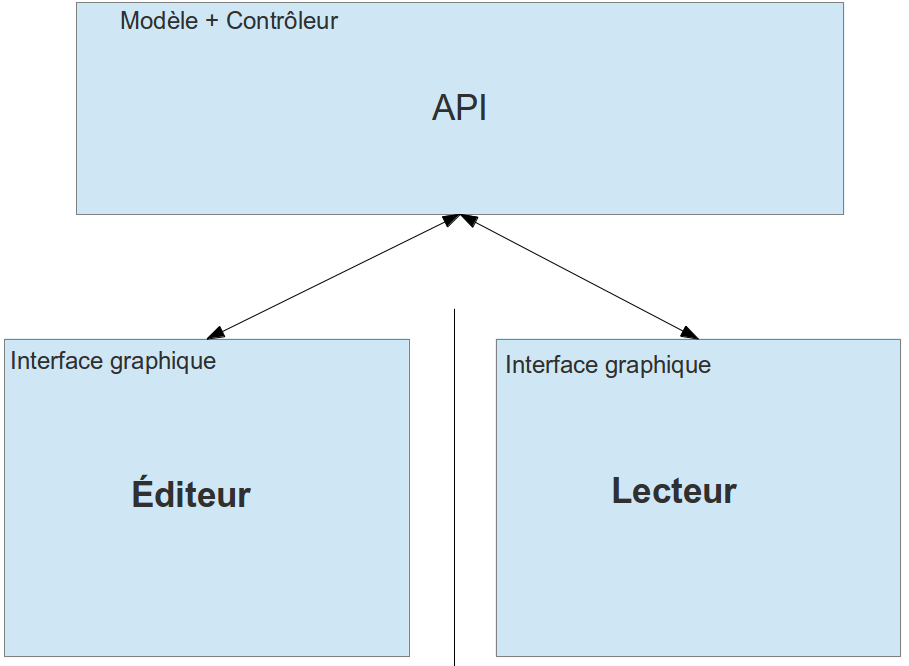
\includegraphics[width=300px]{mvc.png}
\caption{Le modèle MVC dans notre code}
\label{mvc}
\end{center}
\end{figure}


A un autre niveau, nous avons, lorsque c'était facilement appliquable, utilisé le paradigme \ac{MVC} de Qt, ce qui est facilité
par l'utilisation de QtCreator, l'IDE fourni avec Qt. En effet, ce dernier permet de concevoir l'interface graphique directement, et de générer automatiquement le code qui y correspond sans que l'on ait à y toucher, ce qui nous permet de nous concentrer uniquement sur la logique sous-jacente.

On peut notamment s'en rendre compte dans les classes \texttt{TrackProperties} ou \texttt{PartSetter} de l'éditeur.
\subsubsection{L'\ac{API}}

L'\ac{API} a été mise en place dès le début du projet, en regroupant dans un même dossier tous les fichiers sources qui ne concernaient pas directement l'interface graphique du lecteur, ni celle de l'éditeur.

\subsubsection*{La modélisation des accords}

Nous avons ensuite ajouté de nouvelles classes pour modéliser les accords de manière la plus abstraite possible, afin de respecter au mieux les objets Modèle du \ac{MVC}. Nous avons pour cela utilisé trois classes (Tonality, Enrichment, Chord), ainsi que deux énumérations (Note et Alteration) pour définir un accord selon le schéma suivant:
\begin{itemize}
 \item Une \textcolor{blue}{tonalité}, c'est une \textcolor{red}{note} et une \textcolor{green}{altération}: \textcolor{red}{A}\textcolor{green}{$\sharp$}, \textcolor{red}{C}\textcolor{green}{$\flat$}, \textcolor{red}{G}\textcolor{green}{$\natural$}, \dots
 \item Un accord, c'est une \textcolor{blue}{tonalité} et un \textcolor{magenta}{mode}: \textcolor{blue}{G$\flat$}\textcolor{magenta}{m}, \textcolor{blue}{B$\sharp$}\textcolor{magenta}{M}, \dots
\end{itemize}

Cette découpe des modèles se répercute dans l'architecture de ces classes (voir le diagramme de classes de la figure \ref{diag_api_chords}). Bien sûr, différentes méthodes ont été implémentées pour chacune de ces classes, bien qu'en réalité peu d'entre elles soient réellement utilisées par GuitarTutor. C'était néanmoins un bon moyen de repartir sur de bonnes bases au début du projet, et certaines de ces méthodes nous ont finalement été utiles plus tard dans la phase de développement. C'est pourquoi nous avons décidé de les laisser dans l'\ac{API}, dans le cas probable qu'elles soient utiles plus tard à GuitarTutor.

\begin{figure}[H]
\begin{center}
\begin{tikzpicture}
\umlclass[x=-7, y=0]{Chord}{
}{}
\umlclass[x=-13, y=-3]{Enrichment}{
}{}
\umlclass[x=-1, y=-3]{Tonality}{
}{}
\umlclass[x=-1, y=-6]{Note}{
}{}
\umlclass[x=-7, y=-6]{Alteration}{
}{}

\umlunicompo[]{Chord}{Enrichment}
\umlunicompo[]{Chord}{Tonality}
\umlunicompo[]{Tonality}{Alteration}
\umlunicompo[]{Tonality}{Note}
\end{tikzpicture}
\caption{La modélisation des accords dans l'\ac{API}}
\label{diag_api_chords}
\end{center}
\end{figure}

\subsubsection*{La classe \textit{LogicalTrack} et les classes associées}

Ultérieurement, c'est la classe \textit{LogicalTrack} que nous avons mise en place. Cet objet représente en mémoire une grille d'accords. Elle est utilisée par l'éditeur, qui transforme les données entrées par l'utiliseur en une instance de \textit{LogicalTrack}, puis fais la conversion en un fichier XML; et de l'autre côté, elle est utilisée par le lecteur qui initialise un objet \textit{LogicalTrack} à partir de la lecture d'un fichier XML. Sa structure est relativement simple et correspond parfaitement à celle que nous avons choisie d'adopter pour les fichiers XML de sauvegarde de grilles (le format est expliqué plus en détail dans la partie \ref{xml}):
\begin{itemize}
 \item Une grille est une suite de parties (intro, refrain, couplet 1,\dots).
 \item Chaque partie est composée d'une suite de notes
 \item A chaque note correspond un temps de début, le temps de fin étant le début de la note suivante
\end{itemize}

Là encore, le découpage des classes découle parfaitement de cette vision d'une grille (figure \ref{diag_api_tracks}). Parallèlement, la classe \textit{TrackLoader}, elle aussi dans l'\ac{API}, contient deux méthodes statiques qui permettent la conversion d'une instance de \textit{LogicalTrack} vers un fichier XML, ou inversement.

\begin{figure}[H]
\begin{center}
\begin{tikzpicture}
\umlclass[x=-13, y=0]{LogicalTrack}{
}{}
\umlclass[x=-7, y=0]{PartTrack}{
}{}
\umlclass[x=-1, y=0]{TrackChord}{
}{}

\umlunicompo[]{LogicalTrack}{PartTrack}
\umlunicompo[]{PartTrack}{TrackChord}
\end{tikzpicture}
\caption{Modélisation d'une grille d'accords dans l'\ac{API}}
\label{diag_api_tracks}
\end{center}
\end{figure}

\subsubsection*{Les autres rôles de l'\ac{API}}

Comme évoqué en introduction de cette partie, l'\ac{API} a été à la base construite sur les parties du code d'origine n'étant pas directement liées à l'interface. C'est en suivant ce principe que nous avons ajouté à l'\ac{API} la bibliothèque IScoreLight, qui servait à la lecture de grilles d'accord, ainsi que EHPCP qui est utilisée pour la reconnaissance des accords. Dans la même veine, on peut évoquer les classes qui servaient déjà à la gestion audio du lecteur, telles que \textit{Track} (que nous avons plus tard adaptée à nos besoins) pour charger en mémoire un fichier audio, ou \textit{MusicManager}, classe pilier concernant la gestion des entrées et des sorties audio.

\subsubsection{L'éditeur}

Le rôle de l'éditeur est d'assister l'utilisateur pour construire une grille d'accords qui soit lisible et jouable sur le lecteur. En accord avec la conception \ac{MVC}, l'éditeur en lui-même ne regroupe que les éléments se rapportant à l'interface graphique ou ayant des rôles de contrôleurs. La souche de l'éditeur est en fait le widget \textit{GridEditor}, qui sert à la fois d'interface et d'orchestrateur entre les différentes sous-composantes de l'éditeur, à savoir:
\begin{itemize}
 \item \textit{ChordTableWidget}, qui apparaît à l'écran comme un tableau où chaque case (instances de la classe \textit{CaseItem}) doivent contenir un accord
 \item \textit{AudioWindow}, qui regroupe tout ce qui a trait à la synchronisation entre les accords de la grille et le morceau qui sera joué simultanément dans le lecteur.
 \item \textit{TrackProperties}, qui sert à concentrer toutes les informations générales sur la grille en cours d'édition, telles que le nom de l'artiste, la signature rythmique, etc.
\end{itemize}

La classe \textit{GridEditor} orchestre donc l'ensemble des actions de l'utilisateur sur chacune de ces sous-composantes en répercutant les effets sur les autres composantes. Par exemple, changer le nombre d'accords par mesure dans \textit{TrackProperties} va changer l'affichage du \textit{ChordTableWidget}; ou encore, changer le tempo dans l'objet \textit{AudioWindow} va décaler les temps de chaque \textit{CaseItem}.


\begin{figure}[H]
\begin{center}
\begin{tikzpicture}
\umlclass[x=-7, y=0]{GridEditor}{
}{}
\umlclass[x=-13, y=-3]{ChordTableWidget}{
}{}
\umlclass[x=-5, y=-3]{AudioWindow}{
}{}
\umlclass[x=-1, y=0]{TrackProperties}{
}{}
\umlclass[x=-13, y=-6]{CaseItem}{
}{}
\umlclass[x=-10,y=-6]{AudioSync}{
}{}
\umlclass[x=-5,y=-6]{SimpleMusicPlayer}{
}{}
\umlclass[x=0,y=-6]{Waveform}{
}{}

\umlunicompo[]{GridEditor}{ChordTableWidget}
\umlunicompo[]{GridEditor}{AudioWindow}
\umlunicompo[]{GridEditor}{TrackProperties}
\umlunicompo[]{ChordTableWidget}{CaseItem}
\umlunicompo[]{AudioWindow}{AudioSync}
\umlunicompo[]{AudioWindow}{SimpleMusicPlayer}
\umlunicompo[]{AudioWindow}{Waveform}
\end{tikzpicture}
\caption{Diagramme de classes synthétique de l'éditeur}
\label{diag_editor}
\end{center}
\end{figure}

\subsubsection{Le lecteur}

Le but du lecteur est de créer un environnement ludique pour jouer les grilles qui auront préalablement été éditées depuis l'éditeur. Contrairement à l'éditeur, le lecteur est destiné à la fois aux professeurs \textit{et} aux élèves de l'école de musique. Il fallait donc prendre en compte cet élément, notamment lors de la construction de l'interface.

Le déroulement d'une partie est relativement simple:
\begin{itemize}
 \item L'utilisateur indique un fichier XML à ouvrir
 \item Le fichier XML est converti en une LogicalTrack
 \item Le contrôleur initialise l'interface ainsi que les entrées et sorties audio en fonction de la LogicalTrack créée
 \item La partie commence, il ne reste qu'à synchroniser les informations retenues sur l'interface (mise en pause, \dots), sur la musique (passage à l'accord suivant, \dots) et l'entrée audio (reconnaissance d'un accord, \dots) les unes avec les autres
\end{itemize}

C'est la classe \textit{Controler} qui a pour rôle d'orchestrer le lecteur, ce qui explique son rôle central dans le diagramme de classes (figure \ref{diag_player}).

\begin{figure}[H]
\begin{center}
\begin{tikzpicture}
\umlclass[x=-7, y=0]{Controler}{
m\_track : LogicalTrack *}{}
\umlclass[x=-13, y=-3]{PlayerScene}{
}{}
\umlclass[x=-1, y=-3]{SongManager}{
}{}
\umlclass[x=-1, y=0]{Configuration}{
}{}
\umlclass[x=-13, y=-6]{ScrollingItem}{
}{}
\umlclass[x=-9,y=-6]{EntireSong}{
}{}
\umlclass[x=-1,y=-6]{MusicManager}{
}{}

\umlunicompo[]{Controler}{PlayerScene}
\umlunicompo[]{Controler}{SongManager}
\umlunicompo[]{Controler}{Configuration}
\umlunicompo[]{PlayerScene}{EntireSong}
\umlunicompo[]{PlayerScene}{ScrollingItem}
\umlunicompo[]{SongManager}{MusicManager}
\end{tikzpicture}
\caption{Diagramme de classes synthétique du lecteur}
\label{diag_player}
\end{center}
\end{figure}

\subsection{Performance}
Il est nécessaire de distinguer les problèmes de performance dans deux cas :

\begin{itemize}
	\item L'affichage
	\item Les calculs sous-jacents
\end{itemize}

\subsubsection{Performance de l'éditeur}
L'éditeur ne pose pas vraiment de problèmes au niveau des performances: ne sont utilisées que des
objets de base de Qt en grande majorité, ce qui fait que les performances sont directement dépendantes du niveau
d'optimisation de Qt (qui, dans la majorité des cas, s'exécute aussi rapidement qu'une application native).

La seule exception est pour le dessin de la forme d'onde du morceau. Il faut en effet synthétiser une très grande quantité de données dans
une zone réduite, tout veillant à ce que le zoom et le déplacement restent fluides.

Par exemple, un fichier audio qui dure 3 minutes et qui est échantillonné à 44100 Hz (le standard des CD Audio)
nécessitera $44100 * 3 * 60 = 7938000$ échantillons. Il faut trouver un moyen d'afficher de manière lisible ces
échantillons dans les dimensions de la forme d'onde (par défaut 500 pixels de large environ).

L'algorithme utilisé est très simple : on lit dans la copie en mémoire du morceau un groupe de 32 échantillons
(cette valeur a été déterminée de manière empirique en comparant la lisibilité des résultats) qui correspond à la position de
chaque pixel, puis on met dans un tableau qui a pour taille la largeur en pixels de la forme d'onde le maximum sur ce groupe.

Enfin, on effectue un lissage par moyennage sur le tableau obtenu.

\subsubsection{Performance du lecteur}

Le lecteur est beaucoup plus complexe que l'éditeur. D'une part, l'affichage prend un certain temps (que nous avons réduit grâce à l'utilisation d'OpenGL),
et d'autre part, le calcul de la transformée de Fourier dans la librairie EHPCP est intense.

Nous avons effectué des mesures sur le logiciel et avons trouvé que 60\% environ du temps de calcul
passait dans le calcul d'exponentielles complexes dans l'algorithme Butterfly utilisé pour la transformée de Fourier (voir figure \ref{player_performance}).

\begin{figure}[H]
\begin{center}
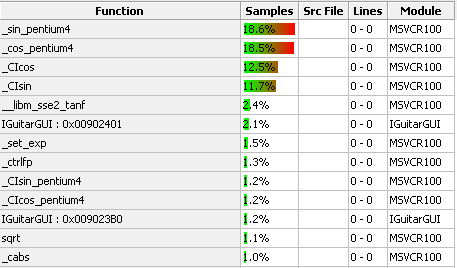
\includegraphics[width=300px]{sincos.png}
\caption{Temps passé par fonction. Données obtenues avec Luke Stackwalker, sous Windows.}
\label{player_performance}
\end{center}
\end{figure}

Les fonctions sin et cos sont en fait issues du simple calcul $e^{ix} = cos(x) + i*sin(x)$.
Elles sont disponibles sous plusieurs formes car les optimisations du compilateur (\ac{MSVC} ici) ont été activées dans leur niveau maximal (avec l'option \texttt{-O2}).

Or, après étude du code, il est apparu que les exponentielles calculées ont toujours des paramètres connus :
\begin{figure}[H]
\begin{lstlisting}
x = (double) ((i%d)*(n/(2*d)));
w = cexp(-I*(2*M_PI*x) / n );
\end{lstlisting}
\caption{Calcul d'exponentielle complexe, extrait de \texttt{fft.c : butterfly}}
\label{api_cexp}
\end{figure}

Ici, i, d et n sont des entiers. Une manière possible d'améliorer de manière drastique les performances serait donc d'effectuer
un pré-calcul de ces facteurs, et de les mettre dans un dictionnaire qui serait appelé par la suite.

Ceci dit, pour améliorer temporairement les performances, nous avons tenté d'utiliser OpenMP dans la dernière boucle qui calcule
les coefficients Butterfly, ce qui permet d'utiliser les capacités des processeurs multicoeur si l'ordinateur cible en dispose. Néanmoins, cela ne fonctionne que sous Linux avec \ac{GCC} et Windows avec \ac{MSVC}, mais pas sous Mac OS X avec Clang.

\subsection{Chronologie de l'architecture de notre logiciel}

\scalebox{1}{
\begin{tabular}{r |@{\hspace{-2.3pt}$\bullet$ \hspace{5pt}} l}

Début du projet & Editeur et lecteur séparés, pas d'\ac{API}, pas multiplateforme.\\
Fin Novembre & Création de l'\ac{API}, ajout de FMOD dans l'\ac{API} pour l'éditeur. \\
Mi-Décembre & Portage Windows, ajout de BOOST. L'éditeur utilise l'\ac{API} et exporte en XML.\\
Début Janvier & Portage Mac OS X. Début de la conception de l'interface du lecteur.\\
Début Février & Passage à Qt5, suppression de BOOST.\\
Mi-Février & Compilation native sous Windows.\\
Fin Février & Suppression de IScoreLight et création d'un nouveau manager pour le lecteur.\\
Début Mars & Le lecteur utilise entièrement l'\ac{API}.\\
Mi-Mars & Suppression de libsndfile, avantageusement remplacé par FMOD dans le lecteur.\\
Fin Mars & Utilisation de Clang sur Mac OS X, \ac{MSVC} sur Windows.\\

\end{tabular}
}
